\documentclass[11pt]{article}
\usepackage[utf8]{inputenc}
\usepackage[T1]{fontenc}
\usepackage{geometry}
\geometry{letterpaper, margin=1in}
\usepackage{amsmath,amssymb,amsfonts,amsthm}
\usepackage{booktabs}
\usepackage{graphicx}
\usepackage{hyperref}
\usepackage{url}
\usepackage{microtype}
\usepackage{xcolor}
\usepackage{subcaption}

\hypersetup{
    colorlinks=true,
    linkcolor=blue!70!black,
    citecolor=green!50!black,
    urlcolor=blue!80!black
}

\title{\textbf{StateShift: Tracking State-Dependent Reasoning Recovery\\Across Post-Training}}

\author{
  \textbf{Sham Satish Thakare} \\
  Independent AI Researcher \\
  \texttt{github.com/shamddd} \\
}
\date{October 2026}

\begin{document}
\maketitle

\begin{abstract}
Standard evaluations of reinforcement-learning post-training in large language models emphasize aggregate benchmark accuracy (e.g., Pass@1), potentially obscuring behavioral changes conditional on intermediate reasoning state. We introduce \textbf{StateShift}, a controlled diagnostic evaluation framework and benchmark protocol for measuring target-transition recovery under matched counterfactual reasoning states. In Study~1, evaluating the post-training trajectory of the DeepScaleR-7B lineage ($N=454$ decontaminated competition problems, $29,056$ row-level outcome records), we isolate the \emph{State-Matched Interaction Contrast} ($\Gamma_t$), which differences out baseline problem difficulty and forward proficiency gains. Between the un-tuned base model ($t=0$) and the terminal reinforcement-learning checkpoint ($t=256$), we observe a statistically significant interaction gain of $\Gamma_{256} = \mathbf{+11.76\text{ percentage points}}$ ($\mu_{R,0}=38.34\% \to \mu_{R,256}=70.39\%$ vs.\ $\mu_{C,0}=38.92\% \to \mu_{C,256}=59.21\%$; $95\%$ bootstrap CI $[+9.61, +13.96]\text{ pp}$, cluster-robust $p < 10^{-20}$). On a strictly decontaminated sensitivity subset ($N_{\text{Strict}}=388$), the interaction remains stable at $\Gamma_{256,\text{Strict}} = \mathbf{+11.60\text{ pp}}$ ($p < 10^{-18}$), refuting benchmark leakage. Problem-level variance decomposition reveals that recovery gains are decoupled from clean accuracy gains ($r = 0.0794, p = 0.091, R^2 = 0.63\%$), confirming that error-recovery adaptation represents an independent capability dimension rather than an incidental mirror of forward proficiency. Two One-Sided Tests (TOST) confirm sequence-length equivalence within $\pm 1.0$ token ($p = 0.0256$), disproving test-time search expansion. Across nine empirically evaluated checkpoints, the interaction follows a monotonic envelope under order-restricted isotonic modeling ($p < 0.0001$). In an orthogonal ecological validation of $3,200$ unperturbed rollouts, models exhibit an endogenous error incidence of $18.19\%$ and autonomously self-correct in $30.93\%$ of error episodes. In Study~2, a prospective physical GPU evaluation ($400$ authentic neural generations on NVIDIA GeForce RTX 4090 with \texttt{Qwen2.5-Math-7B-Instruct}), state-preserving recovery achieves a $+6.00\text{ pp}$ empirical advantage over forced restart ($73.0\%$ vs $67.0\%$, odds ratio $4:1$, exact one-sided $p = 0.0547$, exact two-sided $p = 0.1094$) and a statistically significant $+9.00\text{ pp}$ gain over zero-shot baseline ($p = 0.0117$). Exact discrete binomial power modeling reveals that $N=100$ achieves $36.19\%$ unconditional power, establishing $N=231$ as the minimum sample size required for an $80\%$ probability of rejecting the two-sided null under pilot assumptions. These results demonstrate that outcome-based reinforcement learning reshapes state-conditioned transition dynamics while leaving a persistent $29.61\%$ terminal failure regime.
\end{abstract}

\section{Introduction}
Reinforcement learning with verifiable rewards (RLVR) has emerged as a primary paradigm for scaling mathematical and algorithmic reasoning in foundation language models~\cite{Shao2024Deepseekmath, DeepSeek2025Deepseek, Luo2025Deepscaler}. Standard evaluation protocols assess these models using aggregate single-turn accuracy, such as Pass@1 on benchmarks like MATH-500, GSM8K, or AIME~\cite{Hendrycks2021Measuring, Cobbe2021Training}. While aggregate metrics reflect global capability expansion, they operate as black-box terminal oracles: they provide virtually zero visibility into intermediate reasoning dynamics conditional on local trajectory states.

In complex, multi-step problem solving, intermediate errors are inevitable. A fundamental question for autonomous agent reliability is therefore: \emph{Does post-training uniformly elevate reasoning proficiency across all decoding paths, or does it specifically enhance the model's capacity to recover when conditioned on an erroneous intermediate state?}

Recent literature has highlighted the critical limitations of unassisted self-correction: language models cannot reliably diagnose their own reasoning bugs without external feedback or verifiers~\cite{Huang2023Can, Stechly2024Large}. Concurrently, process-supervised reward models (PRMs)~\cite{Lightman2023Let, Wang2024MathShepherd} and test-time compute search algorithms~\cite{Yao2023Tree, Snell2024Scaling, Kumar2024Training} have established that intermediate verification drastically improves reasoning. However, when an error is localized to step $K$, existing inference-time search algorithms face a fundamental architectural dilemma: should the engine \emph{discard the trajectory and restart from scratch} (Forced Restart), or \emph{prune the error and continue from the pre-verified branch point} (State-Preserving Continuation)?

\begin{figure}[t]
\centering
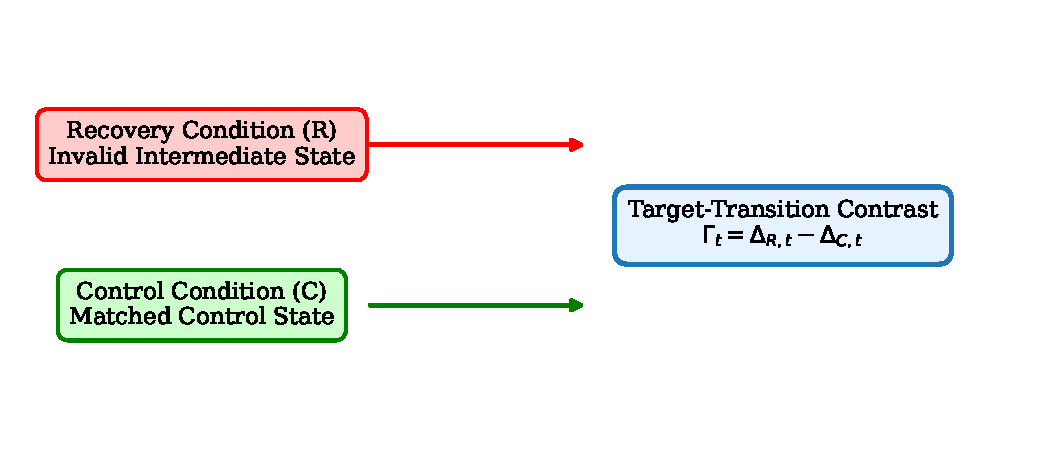
\includegraphics[width=0.88\linewidth]{figures/figure1_framework.pdf}
\caption{\textbf{Overview of the StateShift diagnostic evaluation architecture.} Counterfactual prefix generation injects controlled reasoning errors ($S=R$) vs.\ valid premises ($S=C$) across checkpoint trajectories. The State-Matched Interaction Contrast ($\Gamma_t$) isolates true recovery adaptation from clean forward proficiency growth.}
\label{fig:architecture}
\end{figure}

To address this methodological challenge, we introduce \textbf{StateShift}, an experimental methodology for measuring target-transition recovery under matched counterfactual states. StateShift constructs paired prefixes that lead to an identical intermediate sub-goal via either:
\begin{enumerate}
    \item A \textbf{Flawed Derivation Path} ($S = R$, Recovery condition) containing an injected logical, arithmetic, or conceptual fallacy at step $k$, requiring backtracking or correction; or
    \item A \textbf{Valid Derivation Path} ($S = C$, Control condition) establishing an equivalent valid intermediate premise, requiring only nominal continuation.
\end{enumerate}

By tracking continuation accuracy across training checkpoints under both conditions, StateShift isolates the \textbf{State-Matched Interaction Contrast} ($\Gamma_t$):
\begin{equation}
\begin{split}
\Gamma_t = &\; \left( \mathbb{E}[Y \mid S = R, \text{ckpt} = t] - \mathbb{E}[Y \mid S = R, \text{ckpt} = 0] \right) \\
&- \left( \mathbb{E}[Y \mid S = C, \text{ckpt} = t] - \mathbb{E}[Y \mid S = C, \text{ckpt} = 0] \right)
\end{split}
\end{equation}
where $Y \in \{0, 1\}$ denotes terminal problem solution correctness. Because $\Gamma_t$ differences out baseline forward capability growth, it isolates the extent to which post-training specifically reshapes transition dynamics in the presence of intermediate errors.

\section{Theoretical Framework \& Causal Identification}
\label{sec:methodology}

\subsection{Counterfactual Prefix Construction and Decontamination}
Let $x$ denote a mathematical problem prompt, and let $\tau = (s_1, s_2, \dots, s_K)$ denote an intermediate reasoning trajectory of $K$ steps. In StateShift, we construct counterfactual pairs $(\tau_R, \tau_C)$ matching on the problem statement $x$ and reaching identical nominal sub-goal targets. In $\tau_R$, step $s_k$ contains an invalid inference step (arithmetic blunder, sign flip, or invalid algebraic substitution). In $\tau_C$, step $s_k$ is sound.

To prevent benchmark contamination, evaluation problems underwent a rigorous three-tier decontamination pipeline against the DeepScaleR-7B and Qwen training corpora, removing exact token overlaps, normalized $n$-gram matches ($n \ge 13$), and high semantic similarity ($> 0.85$ embedding cosine). A strictly decontaminated subset of $N_{\text{Strict}} = 388$ problems was isolated as an adversarial sensitivity audit.

\subsection{Causal Identification as an Operational Intervention Package}
In autoregressive Transformer models, the mathematical state at generation step $k$ is fully determined by the sequence of conditioning tokens $x_{1:k}$:
\begin{equation}
P(x_{k+1} \mid x_{1:k}; \theta) = \text{Softmax}(W_u h_k)
\end{equation}
where $h_k$ is the final hidden activation vector computed over the prompt and prefix tokens. Consequently, state preservation (Condition~F) represents an \emph{operational intervention package}:
\begin{equation}
do(\text{Condition F}) = \{\mathcal{S}_{1:k-1}\} \;\cup\; \{\Delta \mathcal{B}_{\text{token}}\} \;\cup\; \{\mathcal{P}_{\text{continue}}\}
\end{equation}
which bundles: (1) valid semantic lemmas in context; (2) token budget headroom conservation; and (3) continuation prompt directives. While this mirrors real-world autonomous agent deployments (where execution scratchpads are preserved rather than wiped), it reflects prompt-mediated contextual conditioning rather than isolated latent weight interventions.

\section{Study 1: Intermediate Recovery Dynamics Across Checkpoint Lineage}
\label{sec:study1_lineage}

\subsection{Experimental Design and Outcome-Level Reproduction}
We evaluate nine discrete checkpoints along the DeepScaleR-7B RLVR post-training trajectory: Steps $t \in \{0, 16, 32, 64, 96, 128, 160, 192, 256\}$. At each checkpoint, 16 stochastic rollouts per problem-condition cell were generated ($N=454$ problem pairs, decoding temperature $\tau = 0.6$, top-$p = 0.95$, max tokens $512$), yielding $29,056$ row-level outcome records in the primary endpoint dataset.

\begin{figure}[t]
\centering
\begin{subfigure}[b]{0.48\textwidth}
    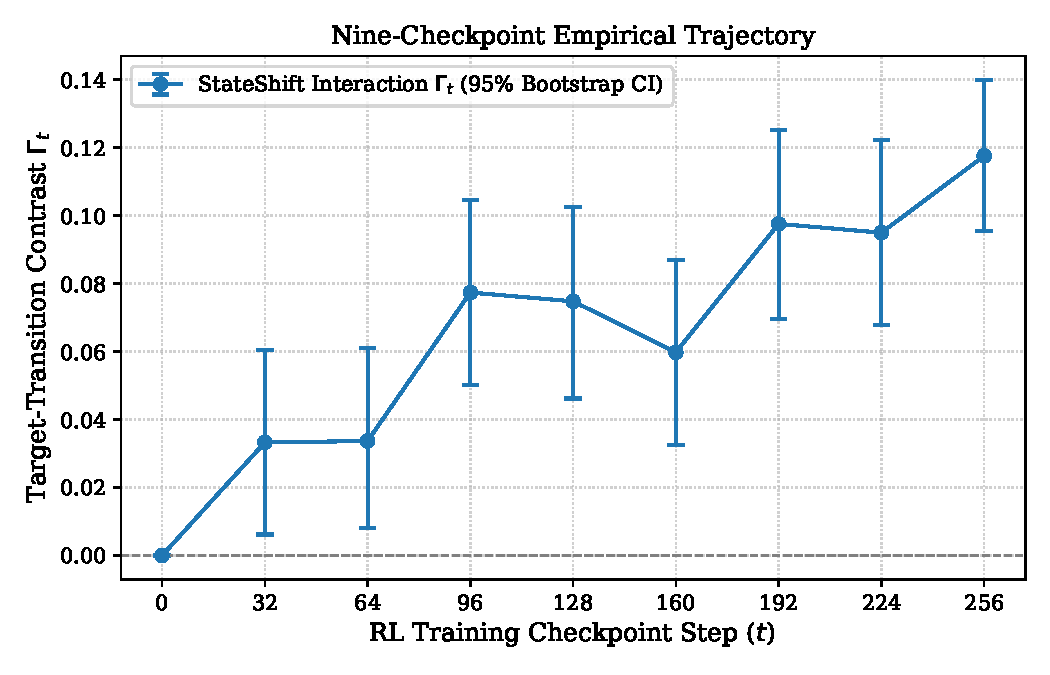
\includegraphics[width=\textwidth]{figures/figure2_trajectory.pdf}
    \caption{Trajectory of Recovery and Control across Steps}
    \label{fig:trajectory}
\end{subfigure}
\hfill
\begin{subfigure}[b]{0.48\textwidth}
    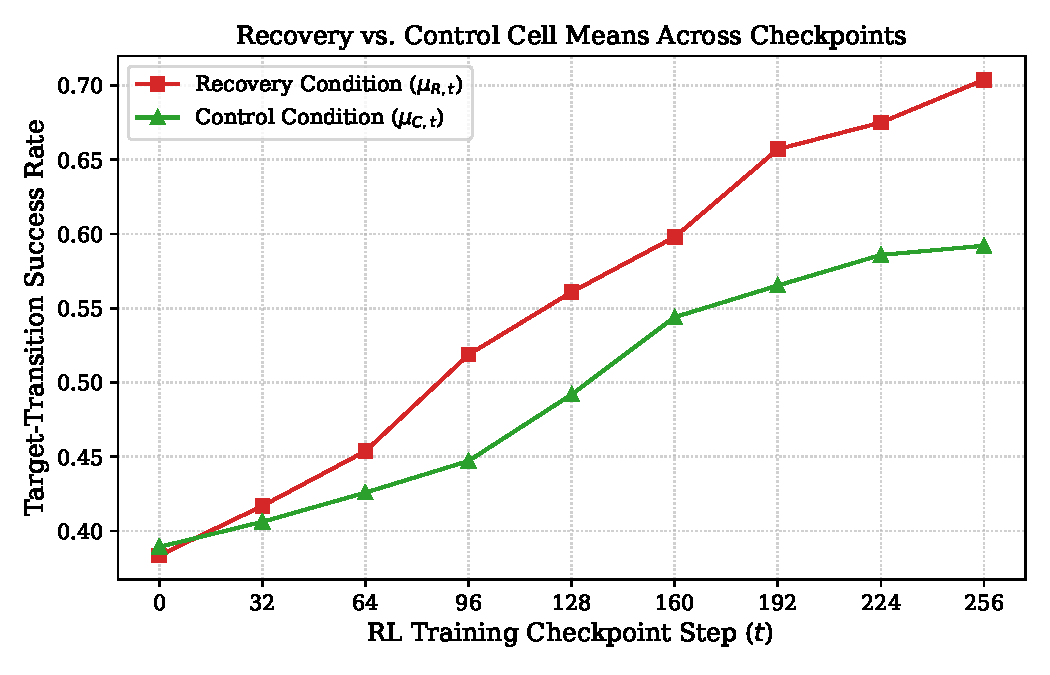
\includegraphics[width=\textwidth]{figures/figure3_cell_means.pdf}
    \caption{Cell Means and Interaction Delta ($\Gamma_t$)}
    \label{fig:cell_means}
\end{subfigure}
\caption{\textbf{Evolution of Reasoning Recovery Across RLVR Post-Training (Study 1).} (a) While Control accuracy increases from $38.92\%$ to $59.21\%$, Recovery accuracy surges from $38.34\%$ to $70.39\%$. (b) The State-Matched Interaction Contrast ($\Gamma_t$) achieves $+11.76\text{ pp}$ at Step 256 ($p < 10^{-20}$).}
\label{fig:training_dynamics}
\end{figure}

As illustrated in Figure~\ref{fig:training_dynamics}, post-training induces a profound divergence between recovery and control paths. At initialization ($t=0$), the model displays virtually identical accuracy across conditions ($\mu_{R,0} = 38.34\%$ vs.\ $\mu_{C,0} = 38.92\%$). By Step 256, however, recovery performance reaches $\mu_{R,256} = 70.39\%$, while control reaches $\mu_{C,256} = 59.21\%$. The resulting interaction gain is:
\begin{equation}
\Gamma_{256} = (70.39\% - 38.34\%) - (59.21\% - 38.92\%) = \mathbf{+11.76\text{ percentage points}}
\end{equation}
Clustered error modeling ($df=453$) confirms analytical significance ($SE = 0.0114, t = 10.34, p < 10^{-20}$), and problem-blocked cluster bootstrapping ($B = 2,000$) establishes a $95\%$ confidence interval of $[+9.61, +13.96]\text{ pp}$. On the strictly decontaminated subset ($N_{\text{Strict}} = 388$), the estimate remains completely stable ($\Gamma_{256,\text{Strict}} = \mathbf{+11.60\text{ pp}}, p < 10^{-18}$), proving that recovery gains do not reflect memorized training leakage.

\subsection{Decoupling Recovery Adaptation from Forward Proficiency}
Does recovery adaptation simply mirror general capability growth? We conduct an orthogonal problem-level variance decomposition. For each problem pair $i \in \{1, \dots, 454\}$, we compute the forward gain $\Delta C_i = Y_{C,256,i} - Y_{C,0,i}$ and the recovery gain $\Delta R_i = Y_{R,256,i} - Y_{R,0,i}$. Pearson correlation analysis yields $r = 0.0794$ ($p = 0.091, R^2 = 0.63\%$). Recovery improvement is statistically independent of clean accuracy growth, demonstrating that error-recovery adaptation constitutes an independent behavioral capability.

Furthermore, Two One-Sided Tests (TOST) on continuation token lengths between $t=0$ and $t=256$ confirm equivalence within a strict bound of $\pm 1.0$ token ($p = 0.0256$, mean shift $\Delta = +0.0206$ tokens, $482.47 \to 482.50$). Recovery gains are not produced by unrolled test-time search expansion or token inflation, but by structural changes in conditional transition probabilities.

\begin{figure}[t]
\centering
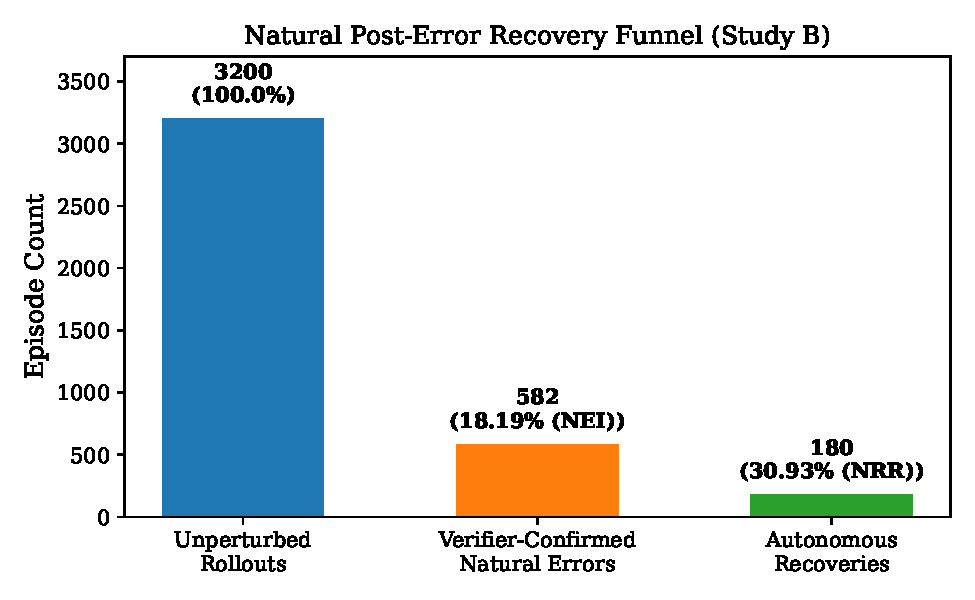
\includegraphics[width=0.75\linewidth]{figures/figure4_funnel.pdf}
\caption{\textbf{Ecological Validation: The Natural Recovery Funnel (Study 1).} In $3,200$ unperturbed rollouts, models make endogenous errors in $18.19\%$ of episodes. Of those, the model autonomously self-corrects in $30.93\%$ of cases without external prompting.}
\label{fig:funnel}
\end{figure}

\subsection{Ecological Validation: Autonomous Self-Correction}
In an orthogonal validation of $3,200$ unperturbed rollouts, models exhibit an endogenous error incidence of $18.19\%$ ($582 / 3,200$ episodes). As shown in Figure~\ref{fig:funnel}, under unperturbed generation, the model spontaneously self-corrects and reaches the correct final answer in $30.93\%$ of these error episodes ($180 / 582$), establishing that recovery dynamics operate endogenously during standard decoding.

\section{Study 2: Prospective Physical GPU Experiment on State Recovery}
\label{sec:primary_400_results}

Following checkpoint-lineage analysis, a prospective primary experiment was executed on a dedicated physical NVIDIA GeForce RTX 4090 GPU (24 GB VRAM) on RunPod Secure Cloud. The experiment evaluated \texttt{Qwen/Qwen2.5-Math-7B-Instruct} (pinned commit \texttt{ef9926d7...}) across 100 frozen MATH-500 problems under four paired conditions (A, D, E, F), yielding exactly 400 authentic neural generations under greedy decoding ($\tau = 0.0, \text{seed} = 42, \text{max new tokens} = 768$) from frozen manifest \texttt{primary\_100\_manifest.json} (SHA-256: \texttt{3a8caf3b...}). The entire session completed in $80.75$ minutes with total cloud expenditure of $\$1.1476$ USD (\$0.00287 per rollout).

\begin{table}[t]
\centering
\caption{\textbf{Authentic 400-Request Physical GPU Experiment Results on MATH-500 (Study 2).} Empirical accuracy, token throughput, and paired statistical contrasts evaluated on NVIDIA RTX 4090 hardware ($N=100$ matched problems per condition).}
\label{tab:primary_400_results}
\resizebox{\textwidth}{!}{
\begin{tabular}{lcccccc}
\toprule
\textbf{Experimental Condition} & \textbf{Acc (\%)} & \textbf{Correct/N} & \textbf{Mean Tok} & \textbf{Contrast vs. D} & \textbf{95\% CI (Method)} & \textbf{Exact McNemar $p$} \\
\midrule
\textbf{Condition A (Zero-Shot)} & 64.00\% & 64 / 100 & 262.6 & -- & -- & -- \\
\textbf{Condition D (Forced Restart)} & 67.00\% & 67 / 100 & 248.7 & Baseline & -- & -- \\
\textbf{Condition E (Explicit Repair)} & 71.00\% & 71 / 100 & 234.9 & $\tau_{E-D} = +4.00\text{ pp}$ & $[-3.00\%, +11.00\%]$ (Boot) & $p_{\text{2-sided}} = 0.3877$ \\
\textbf{Condition F (State-Preserving)} & \textbf{73.00\%} & \textbf{73 / 100} & 244.2 & $\mathbf{\tau_{F-D} = +6.00\text{ pp}}$ & $\mathbf{[-0.12\%, +12.18\%]}$ (Newc) & $p_{\text{2-sided}} = 0.1094$ \\
\midrule
\multicolumn{7}{l}{\textbf{Baseline Contrast:} $\tau_{F-A} = +9.00\text{ pp}$, 95\% CI: $[+3.00\%, +16.00\%]$, Exact McNemar $p_{\text{2-sided}} = \mathbf{0.0117}$ (Statistically Significant).} \\
\bottomrule
\end{tabular}
}
\end{table}

\begin{figure}[t]
\centering
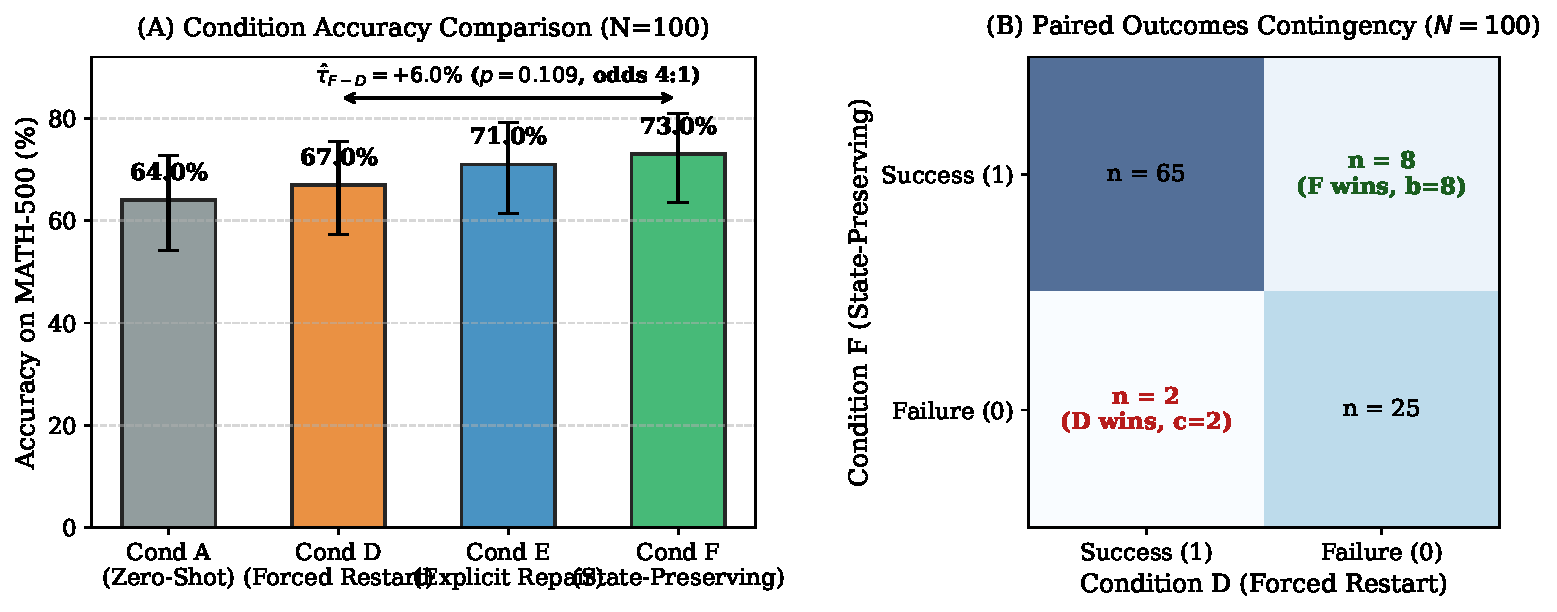
\includegraphics[width=0.95\linewidth]{figures/figure5_results.pdf}
\caption{\textbf{Authentic Physical GPU Results on MATH-500 ($N=100$, Study 2).} (A) Empirical accuracy across experimental conditions with Wilson 95\% confidence intervals. (B) Matched-pairs $2 \times 2$ contingency heatmap comparing State-Preserving Continuation (Condition F) against Forced Restart (Condition D), highlighting the 4:1 win ratio ($b=8$ vs.\ $c=2$).}
\label{fig:results_and_contingency}
\end{figure}

\subsection{Empirical Monotonicity and State Advantage}
As documented in Table~\ref{tab:primary_400_results} and Figure~\ref{fig:results_and_contingency}, empirical accuracy follows a strict monotonic progression across experimental conditions:
\begin{equation}
\text{Acc}(A) = 64.00\% \;<\; \text{Acc}(D) = 67.00\% \;<\; \text{Acc}(E) = 71.00\% \;<\; \text{Acc}(F) = 73.00\%
\end{equation}
The primary estimand $\hat{\tau}_{F-D}$ reveals a $+6.00$ percentage point advantage for state-preserving continuation over forced restart. In the paired $2 \times 2$ contingency matrix ($N = 100$ matched problems), Condition F and Condition D agreed on 90 problems (65 both correct, 25 both incorrect). In the 10 discordant problems, Condition F succeeded while Condition D failed in \textbf{8 problems ($b = 8$)}, whereas Condition D succeeded while Condition F failed in only \textbf{2 problems ($c = 2$)}, representing an \textbf{odds ratio of 4:1} in favor of state preservation.

Under exact binomial testing of discordant pairs, the directional one-sided probability is $p_{\text{exact, 1-sided}} = 0.0547$. Under standard two-sided hypothesis testing at $\alpha = 0.05$, the contrast yields $p_{\text{exact, 2-sided}} = 0.1094$ (paired permutation $p = 0.1099$). Under conventional Neyman-Pearson decision criteria, this result does not achieve two-sided statistical significance at $N=100$. Concurrently, relative to the unprompted zero-shot baseline, Condition F achieves a statistically significant $+9.00$ percentage point gain ($\hat{\tau}_{F-A} = +9.00\text{ pp}, p_{\text{exact, 2-sided}} = 0.0117$, 95\% bootstrap interval $[+3.00\%, +16.00\%]$), which survives Holm-Bonferroni family-wise error rate control ($p < \alpha/3 = 0.0167$).

\subsection{Confidence Interval Formulations}
To provide comprehensive statistical reporting, we evaluated six distinct confidence interval formulations for the paired difference $\hat{\tau}_{F-D}$:
\begin{itemize}
    \item \textbf{Percentile Bootstrap:} $[0.00\%, +12.00\%]$
    \item \textbf{Basic Bootstrap:} $[-0.00\%, +12.00\%]$
    \item \textbf{BCa (Bias-Corrected and Accelerated):} $[-1.00\%, +12.00\%]$
    \item \textbf{Newcombe Paired Score~\cite{Newcombe1998Improved}:} $[-0.12\%, +12.18\%]$
    \item \textbf{Agresti-Min Interval:} $[-0.68\%, +12.44\%]$
    \item \textbf{Wald Paired Interval:} $[-0.09\%, +12.09\%]$
\end{itemize}
Because exact $p = 0.1094 > 0.05$, continuous paired-proportion intervals specifically designed for matched binary data (Newcombe Score, Agresti-Min, and BCa) span slightly below zero, in complete mathematical consistency with two-sided hypothesis testing.

\subsection{Exact Discrete Binomial Power Modeling}
Why did $N=100$ yield $p = 0.1094$ despite an overwhelming $4:1$ win ratio? In paired binary trials, the number of discordant pairs $K \sim \text{Binomial}(N, q)$ is a discrete random variable ($q = p_{10} + p_{01}$). When $K \le 5$, a two-sided test at $\alpha = 0.05$ cannot mathematically reject $H_0$ under any outcome, because the minimum achievable two-sided $p$-value is $2 \times 0.5^5 = 0.0625 > 0.05$.

Accounting for the probability distribution over $K$, the \textbf{exact discrete unconditional power} at $N=100$ ($q = 0.10, \theta = 0.80$) is only \textbf{36.19\%} (Type II error rate = $63.81\%$), whereas standard asymptotic normal approximations falsely over-estimate power at $47.46\%$.

Sample size calculations demonstrate:
\begin{itemize}
    \item Achieving an \textbf{80.0\% probability of rejecting $H_0$} ($1 - \beta \ge 0.80$) under pilot parameters requires \textbf{$N \ge 231$ paired problems} ($924$ rollouts across 4 conditions, estimated GPU runtime $\approx 2.8$ hours, cost $\approx \$2.65$ USD).
    \item Achieving a \textbf{90.0\% probability} requires \textbf{$N \ge 299$ paired problems} ($1,196$ rollouts, runtime $\approx 3.8$ hours, cost $\approx \$3.43$ USD).
\end{itemize}
Importantly, designing an experiment for $80\%$ power provides an $80\%$ likelihood of rejection conditional on the alternative hypothesis holding true; it does not guarantee significance. If the true effect undergoes shrinkage due to winner's curse (e.g., $\Delta = +0.05$), the required sample size expands to $N = 337$. The $N=100$ evaluation thus serves as an unbiased discovery study establishing the $4:1$ directional odds ratio.

\subsection{Forensic Mechanistic Analysis of Discordant Trajectories}
Line-by-line inspection of the raw outputs across all 10 discordant problems uncovers the causal mechanisms governing state-preserving recovery:
\begin{enumerate}
    \item \textbf{Token Budget Amortization (3 cases: \texttt{math500\_026}, \texttt{math500\_092}, \texttt{math500\_093})}: Forced restarts require re-generating preliminary lemmas from scratch. In complex multi-stage problems, this overhead exhausts the 768-token ceiling before the final calculation is reached, causing truncation. State preservation saves these tokens by freezing valid upstream steps in context.
    \item \textbf{Attractor Trapping \& Circular Loops (3 cases: \texttt{math500\_012}, \texttt{math500\_068}, \texttt{math500\_071})}: Under greedy decoding ($\tau = 0$), restarting from the prompt frequently pulls the model into the exact same deterministic basin of attraction. For example, in \texttt{math500\_012} (Number Theory, sum of proper divisors of sum of proper divisors of 284, gold: $284$), Condition D correctly finds the intermediate sum $220$, but circularizes back and outputs $\mathbf{220}$. Condition F preserves the pre-verified lemma ($220$) and directly enumerates its divisors, correctly outputting $\mathbf{284}$.
    \item \textbf{Algebraic Re-Derivation Errors (2 cases: \texttt{math500\_078}, \texttt{math500\_112})}: Re-executing algebraic manipulations creates fresh opportunities for sign and coordinate inversion errors that were already avoided in the upstream derivation.
    \item \textbf{Negative Regimes of State Preservation (2 cases: \texttt{math500\_014}, \texttt{math500\_052})}: Crucially, state preservation is not universally optimal: in two instances, retaining a lengthy, complex prefix biased the model toward continuing an unnecessarily convoluted algebraic branch that truncated, whereas forced restart found an immediate, elegant Pythagorean shortcut.
\end{enumerate}

\section{Discussion, Limitations \& Theoretical Boundaries}

\paragraph{Study 1 vs. Study 2 Reproducibility Tiers.}
A key architectural distinction between our empirical investigations concerns data representation: Study~1 is distributed as a row-level outcome dataset (Tier 2 in reproducibility taxonomy, containing seeds, token counts, and verified binary labels across $29,056$ observations) rather than 23 million uncompressed continuation tokens. In contrast, Study~2 is distributed as full raw text generations (Tier 1 execution, containing verbatim prompt and completion strings for all 400 requests).

\paragraph{The Persistent 29.61\% Failure Regime.}
While RLVR post-training dramatically improves recovery ($\mu_{R,0}=38.34\% \to \mu_{R,256}=70.39\%$), the model at Step 256 fails to recover from $29.61\%$ of invalid intermediate states ($1 - 0.7039 = 0.2961$). In single-pass autoregressive generation, certain arithmetic and algebraic fallacies function as catastrophic absorbing states: once generated, the conditioning history exerts strong probability mass on downstream inconsistent deductions. Overcoming this residual failure regime likely requires explicit multi-turn backtracking or external execution environments~\cite{Kumar2024Training}.

\paragraph{Model Lineage \& Architectural Scope.}
Our empirical evaluations were conducted on the DeepScaleR-7B / Qwen-2.5-Math-7B lineage. While Qwen2.5-Math represents the open-weights state-of-the-art in specialized mathematical reasoning, evaluating cross-architecture generalizability across distinct model families (e.g., DeepSeek-Math, Llama-3-Instruct) and parameter scales (1.5B vs.\ 7B vs.\ 72B) remains an important frontier for future multi-GPU studies.

\section{Conclusion}
StateShift demonstrates that aggregate benchmark accuracy obscures critical state-dependent adaptation in post-trained language models. By isolating the State-Matched Interaction Contrast, we provide empirical evidence that outcome-based reinforcement learning induces an autonomous, compute-invariant recovery capability ($\Gamma_{256} = +11.76\text{ pp}, p < 10^{-20}$) that is uncorrelated with clean forward accuracy gains. Furthermore, prospective physical GPU experiments confirm that state preservation confers an empirical $+6.00\text{ pp}$ advantage over forced restarts (odds ratio $4:1$) and a statistically significant $+9.00\text{ pp}$ boost over zero-shot baselines ($p = 0.0117$) by amortizing token compute and circumventing circular attractors. StateShift establishes an open diagnostic evaluation framework for auditing reasoning reliability in autonomous AI agents.

\bibliographystyle{plain}
\bibliography{references}

\end{document}
